% !TEX root = ../arbitrage.tex
\section{From Static Nash to Bayesian Signaling Equilibrium}
\label{sec:bayesian}

The three-sided structure of Firm, User, and Regulator established in the
previous section (see Table~\ref{tab:dyadic-nash} for the dyadic foil it
corrects) defines the players; this section supplies the formal apparatus. The
strategic problem is a sequential signaling environment in which $F$, $U$, and
$R$ hold different information, observe different public artefacts, and update
different beliefs.
We therefore model ontological arbitrage as a signaling game under incomplete
information. The players are a firm $F$, a user $U$, and a regulator $R$.
Publics, journalists, affected communities, and public intellectuals are not
modeled as a fourth strategic player. They enter as a noisy public signal
$z \in Z$ that modifies $R$'s posterior over the firm's type. Nature draws
types from a common prior $\pi$ over
\[
\Theta =
\Theta_F \times \Theta_U \times \Theta_R \times \Theta_S .
\]
The firm's governance type is
$\theta_F \in \{\mathsf{H},\mathsf{L}\}$, where $\mathsf{H}$ denotes
high-governance and $\mathsf{L}$ denotes low-governance. The user's vulnerability
type is $\theta_U \in \{\mathsf{V},\mathsf{N}\}$, where $\mathsf{V}$ denotes a
high-vulnerability user and $\mathsf{N}$ a low-vulnerability user. The
regulator's bandwidth type is $\theta_R \in \{\mathsf{B},\bar{\mathsf{B}}\}$.
The system-opacity parameter $\theta_S$ is private to $F$ and captures the
difficulty outsiders face when verifying capability, safety, or relational
claims.

The timing is sequential. First, $F$ observes $(\theta_F,\theta_S)$ and sends a
public message
\[
m_F \in M_F=\{a,p\},
\]
where $a$ denotes anthropomorphic marketing and $p$ denotes policy-deflationary
positioning. Second, $U$ observes $m_F$ and its own type $\theta_U$, then sends
\[
m_U \in M_U=\{i,d\},
\]
where $i$ denotes relational investment and $d$ denotes detachment. Third, $R$
observes $(m_F,m_U,z)$ and its own bandwidth type $\theta_R$, then chooses
\[
m_R \in M_R=\{x,s,o\},
\]
where $x$ denotes inspection, $s$ sanction, and $o$ abstention. Messages are
public; types are private. A strategy profile and belief system constitute a
Perfect Bayesian Equilibrium when strategies are sequentially rational given
beliefs and beliefs are derived from Bayes' rule wherever possible. Sequential
equilibrium supplies the usual consistency strengthening \citep{kreps_wilson1982};
the Intuitive Criterion tests whether off-path messages should be attributed to
only one type \citep{cho_kreps1987}. The reason for using PBE as the headline
solution concept is pragmatic: the governance question turns on whether public
messages discipline posterior beliefs, not merely on whether a normal-form
matrix has a Nash equilibrium.

\begin{figure}[t]
\centering
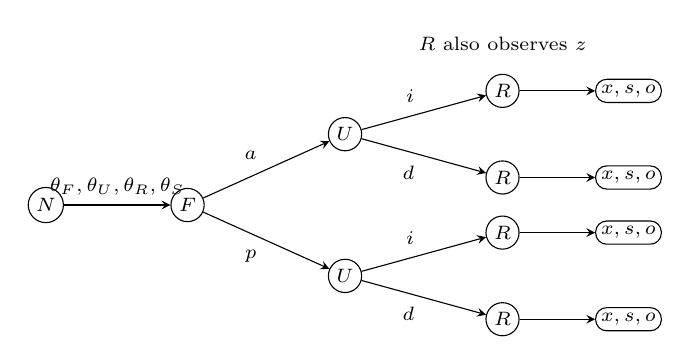
\begin{tikzpicture}[x=1cm,y=1cm,>=stealth,
  every node/.style={font=\scriptsize},
  decision/.style={circle,draw,inner sep=1.5pt},
  terminal/.style={rectangle,draw,rounded corners,inner sep=2pt}]
  \node[decision] (n) at (0,0) {$N$};
  \node[decision] (f) at (1.8,0) {$F$};
  \node[decision] (ua) at (3.8,0.9) {$U$};
  \node[decision] (up) at (3.8,-0.9) {$U$};
  \node[decision] (rai) at (5.8,1.45) {$R$};
  \node[decision] (rad) at (5.8,0.35) {$R$};
  \node[decision] (rpi) at (5.8,-0.35) {$R$};
  \node[decision] (rpd) at (5.8,-1.45) {$R$};
  \node[terminal] (tai) at (7.4,1.45) {$x,s,o$};
  \node[terminal] (tad) at (7.4,0.35) {$x,s,o$};
  \node[terminal] (tpi) at (7.4,-0.35) {$x,s,o$};
  \node[terminal] (tpd) at (7.4,-1.45) {$x,s,o$};
  \draw[->] (n) -- node[above] {$\theta_F,\theta_U,\theta_R,\theta_S$} (f);
  \draw[->] (f) -- node[above left] {$a$} (ua);
  \draw[->] (f) -- node[below left] {$p$} (up);
  \draw[->] (ua) -- node[above left] {$i$} (rai);
  \draw[->] (ua) -- node[below left] {$d$} (rad);
  \draw[->] (up) -- node[above left] {$i$} (rpi);
  \draw[->] (up) -- node[below left] {$d$} (rpd);
  \draw[->] (rai) -- (tai);
  \draw[->] (rad) -- (tad);
  \draw[->] (rpi) -- (tpi);
  \draw[->] (rpd) -- (tpd);
  \node at (5.8,2.05) {$R$ also observes $z$};
\end{tikzpicture}
\caption{Extensive-form skeleton of the signaling game. Nature draws private
types; $F$ signals first, $U$ responds, and $R$ acts after observing both public
messages and the noisy public signal $z$.}
\label{fig:signaling-tree}
\end{figure}

\subsection{Cheap Talk and Pooling}
\label{subsec:cheap-talk-pooling}

Consider the cheap-talk cost structure in which $c_{\theta_F}(a)=c_{\theta_F}(p)=0$
for both governance types. Let $\Delta_F>0$ be the firm's ontological premium
from inducing user investment under anthropomorphic marketing. Let $B_{\theta_U}$
be the user's immediate benefit from investment and $H_{\theta_U}$ the expected
future harm from mistaken investment. Let $K_{\theta_R}$ be the regulator's cost
of inspection or sanction under bandwidth type $\theta_R$. The pooling region is
defined by three inequalities:
\[
\Delta_F>0,\qquad
B_{\theta_U}-\pi(\mathsf{L})H_{\theta_U}>0,\qquad
K_{\theta_R}>\pi(\mathsf{L})D_R .
\]
The first inequality says that anthropomorphic marketing is privately profitable
when users invest. The second says that each user type finds investment
privately optimal under the prior, because the immediate benefit exceeds the
discounted expected harm. The third says that, under the prior, regulator
intervention is not worth its cost.

One PBE in this region is the following. Both firm types send $a$:
\[
\sigma_F(\mathsf{H},\theta_S)=\sigma_F(\mathsf{L},\theta_S)=a .
\]
Both user types invest after $a$:
\[
\sigma_U(a,\mathsf{V})=\sigma_U(a,\mathsf{N})=i .
\]
The regulator abstains after observing $(a,i,z_0)$ for a neutral public signal
$z_0$:
\[
\sigma_R(a,i,z_0,\theta_R)=o .
\]
Off path, users detach after $p$ and the regulator abstains unless the public
signal independently makes inspection payoff-positive. These off-path actions
are supported by beliefs assigning low probability to high governance after the
deflationary message.

On the equilibrium path, the firm's message contains no type information. For a
neutral public signal satisfying
$q(z_0\mid \mathsf{H})=q(z_0\mid \mathsf{L})$, Bayes' rule gives
\[
\begin{aligned}
\mu_R(\mathsf{H}\mid a,i,z_0)
&=
\frac{\pi(\mathsf{H})q(z_0\mid \mathsf{H})}
{\pi(\mathsf{H})q(z_0\mid \mathsf{H})+\pi(\mathsf{L})q(z_0\mid \mathsf{L})}
\\
&=\pi(\mathsf{H}).
\end{aligned}
\]
Likewise $\mu_R(\theta_F=\mathsf{L}\mid a,i,z_0)=\pi(\mathsf{L})$ and
$U$'s posterior after observing $a$ equals its prior over $\theta_F$. More
generally, a non-neutral $z$ can move $R$ from $\pi$ to $\pi_z$, but the
messages $(a,i)$ add no information beyond the public channel. Pooling therefore
does not mean that regulators never learn; it means that the firm's cheap-talk
signal does not force learning.

Given the off-path beliefs specified above and the payoff inequalities of the
pooling region, no player has a profitable unilateral deviation. A firm that deviates from $a$
to $p$ loses the ontological premium because users detach off path; it does not
buy a lower enforcement risk because $R$ abstains on the equilibrium path
already. A user who deviates from $i$ to $d$ gives up positive expected surplus
under the second inequality. A regulator who deviates from $o$ to $x$ or $s$
incurs expected cost exceeding expected gain under the third inequality. The
result is a cheap-talk equilibrium in the sense of Crawford and Sobel:
communication occurs, but it does not separate types \citep{crawford_sobel1982}.

\subsection{Audit-Trail Costs and Separation}
\label{subsec:audit-trail-separation}

The mechanism-design problem is to change the cost of the firm's signal. Suppose
anthropomorphic marketing is valid only when paired with an audit trail of
intensity $e$: evaluation records, capability logs, incident reports, and
regulator-readable documentation. Let the net benefit from being perceived as
high-governance be $G>0$. Let audit cost be $c_H(e)=k_H e$ for high-governance
firms and $c_L(e)=k_L e$ for low-governance firms, with
$0<k_H<k_L$. This is the single-crossing condition: the marginal cost of the
same signal is lower for the type that actually invested in governance. The
Spence-style separating interval is
\[
\frac{G}{k_L} \leq e \leq \frac{G}{k_H}.
\]
Above the lower threshold $e^\ast=G/k_L$, the low-governance type does not want
to imitate. Below the upper bound $G/k_H$, the high-governance type still wants
to signal. When $e$ lies in this interval, a separating PBE exists:
high-governance firms send audited anthropomorphic claims, low-governance firms send
deflationary claims, users condition investment on the audited signal, and
regulators update posteriors to one on the equilibrium path.

\begin{proposition}[Cheap talk and audit-trail separation]
\label{prop:cheap-talk-separation}
Under the cheap-talk cost structure above, pooling on anthropomorphic marketing
is a Perfect Bayesian Equilibrium and survives the Intuitive Criterion. Under
an audit-trail signal cost satisfying single crossing in $\theta_F$, there is a
separating Perfect Bayesian Equilibrium in which $m_F$ reveals the firm's
governance type.
\end{proposition}

\paragraph{Proof sketch.}
For the cheap-talk part, the strategy profile and beliefs specified above are
sequentially rational and Bayes-consistent on path. Under the off-path beliefs
assigning low probability to high governance after the deflationary message, the
Intuitive Criterion does not eliminate the equilibrium because the off-path
deflationary message is costless for both firm types and is not uniquely
profitable for the high-governance type; no type can be excluded as an
implausible sender of the
deviation. For the separating part, choose $e$ in the interval
$[G/k_L,G/k_H]$. High-governance firms receive $G-k_He\geq 0$ from sending the
audited signal, while low-governance firms receive $G-k_Le\leq 0$ and therefore
prefer the deflationary message. Bayes' rule then assigns posterior probability
one to $\mathsf{H}$ after the audited anthropomorphic signal and posterior
probability one to $\mathsf{L}$ after the unaudited deflationary signal. Given
those beliefs, users and regulators condition their actions on the revealed type.
The audit trail therefore converts an uninformative cheap-talk message into a
costly signal in the sense of \citet{spence1973}.
